% --- Main Content ---
\chapter{Introduction}
\label{chap:introduction}

The introduction should provide background information on your topic, explain the significance of your research, and clearly state your research question or objective. This chapter should also outline the structure of the document and briefly summarize each subsequent chapter. 

Times New Roman font is used for the text in this document, and the font size is set to 12pt. The line spacing is set to 1.5 for better readability.

\section{Background}
This section should provide context for your research, explaining fundamental concepts necessary for understanding your work. 
% Artificial Intelligence (\gls{ai}) is a rapidly growing field. Subfields such as \gls{ml} and \gls{nlp} are gaining significant attention.

\section{Motivation}
Explain why your research topic is important and what gap in knowledge it addresses.

\section{Problem Statement}
Clearly articulate the specific problem or question your research aims to address.

\section{Outline of the Report}
Provide a brief overview of the structure of your document, summarizing the content of each chapter.

% CHAPTER 2: LITERATURE REVIEW
\chapter{Literature Review}
This chapter should synthesize existing research relevant to your topic. Analyze the current state of knowledge, identify gaps, and position your research within the existing literature.

\section{Overview of Existing Work}
Summarize key research papers, books, and other sources related to your topic.

\section{Current Trends}
Discuss recent developments and emerging trends in your research area.

\section{Research Gaps}
Identify limitations or gaps in existing research that your work aims to address.

% --- Theoretical Framework ---
% CHAPTER 3: THEORETICAL FRAMEWORK
\chapter{Theoretical Framework}
Present the theoretical foundation of your research, including relevant models, equations, algorithms, or principles.

\section{Key Concepts}
Define and explain the fundamental concepts central to your research.

\section{Mathematical Formulation}
Present any relevant mathematical formulations, theorems, or proofs.

\section{Algorithms}
This section presents the algorithms used in this research.

% Example of how to include an algorithm with proper referencing
Algorithm \ref{alg:example} demonstrates a basic search algorithm. This example shows how to properly format and include algorithms in your document.

\begin{algorithm}
\caption{Binary Search Algorithm}
\label{alg:example}
\begin{algorithmic}[1]
\Procedure{BinarySearch}{$A, n, x$}
    \State $low \gets 1$
    \State $high \gets n$
    \While{$low \leq high$}
        \State $mid \gets low + \lfloor (high - low) / 2 \rfloor$ \Comment{Avoid integer overflow}
        \If{$A[mid] < x$}
            \State $low \gets mid + 1$
        \ElsIf{$A[mid] > x$}
            \State $high \gets mid - 1$
        \Else
            \State \Return $mid$
        \EndIf
    \EndWhile
    \State \Return $-1$
\EndProcedure
\end{algorithmic}
\end{algorithm}

\subsection{Algorithm Complexity Analysis}
When analyzing the time complexity of Algorithm \ref{alg:example}, we find that binary search operates in $O(\log n)$ time, where $n$ is the number of elements in the sorted array. This is because each comparison eliminates approximately half of the remaining elements.

\subsection{Pseudocode Formatting Tips}
When writing algorithms:
\begin{itemize}
    \item Use consistent indentation
    \item Number each line for easy reference with \texttt{algorithmic[1]}
    \item Include proper comments for complex steps
    \item Clearly define inputs and outputs of procedures
\end{itemize}

% IMPORTANT: Always reference every figure in the text BEFORE it appears
Figure \ref{fig:external_image} illustrates a key concept of this research. As shown in the figure, important relationships between variables can be visualized.
As shown in Figure \ref{fig:tikz_figure}, the following diagram illustrates the relationship between key variables.

% Example of adding a referenced figure
\begin{figure}[H]
    \centering
    
\includegraphics[width=0.5\textwidth]{example-image.jpg} % Replace 'sample-figure.jpg' with your image file name
    \caption[Short caption for sample figure]{Detailed caption explaining the sample figure. The short caption appears in the list of figures.}
    \label{fig:external_image}
\end{figure}

% Example of drawing a figure using TikZ
\begin{figure}[H]
    \centering
    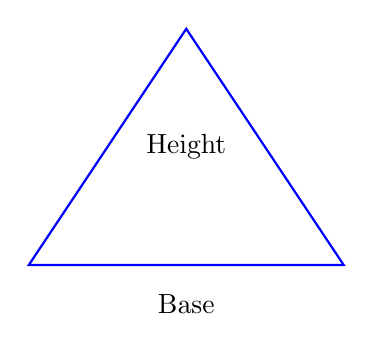
\begin{tikzpicture}
        % Example TikZ drawing: A simple triangle
        \draw[thick, blue] (0,0) -- (4,0) -- (2,3) -- cycle;
        \node at (2,-0.5) {Base};
        \node at (2,1.5) {Height};
    \end{tikzpicture}
    \caption[Short caption for TikZ figure]{Detailed caption explaining the TikZ-drawn figure. The short caption appears in the list of figures.}
    \label{fig:tikz_figure}
\end{figure}

% IMPORTANT: Every figure must be referenced in the text (e.g., "As shown in Figure \ref{fig:label}...")

\section{Example Implementation}
Listing \ref{lst:python_example} demonstrates a Python function implementation that doubles its input parameter. This code sample illustrates how to include formatted code in your document with syntax highlighting.

\begin{lstlisting}[language=Python, caption=Example Python Code, breaklines=true, label=lst:python_example]
def example_function(parameter):
    """
    This is a sample function to demonstrate code inclusion. It takes a parameter and returns its double.
    :param parameter: The input value to be doubled.
    """
    result = parameter * 2
    return result

# Example usage
value = 42
print(f"The result is: {example_function(value)}")
\end{lstlisting}

\subsection{Example Equations}
Below are sample equations formatted in LaTeX:

% Inline equation example
The quadratic formula $ax^2 + bx + c = 0$ has the solution $x = \frac{-b \pm \sqrt{b^2 - 4ac}}{2a}$.

% Display equation example
\begin{equation}
    E = mc^2
\end{equation}

% Equation array example
\begin{align}
    (a+b)^2 &= a^2 + 2ab + b^2\\
    (a-b)^2 &= a^2 - 2ab + b^2
\end{align}

% --- Methodology ---
% CHAPTER 4: METHODOLOGY
\chapter{Methodology}
Describe your research approach, methods, experimental setup, and data collection procedures.

\section{Research Approach}
Explain the overall approach or strategy you used in your research.

\section{Experimental Setup}
Describe the equipment, materials, or software used in your research.

\section{Data Collection}
Explain how you collected data, including any sampling strategies or selection criteria.

\section{Analysis Methods}
Describe the statistical techniques or analytical methods you used to process and interpret your data.

% --- Results and Discussion ---
% CHAPTER 5: RESULTS AND DISCUSSION
\chapter{Results and Discussion}
Present your findings and interpret them in the context of your research question and existing literature.

\section{Key Findings}
Describe the main results of your research, supported by data, figures, or tables.

% IMPORTANT: Notice that the table is referenced in the text BEFORE it appears
% Always reference tables in your text before they are displayed
Table \ref{tab:sample_table} presents the sample data collected during the experiment.

\begin{table}[ht]
    \centering
    \caption{Sample Table Format}  % Table caption
    \label{tab:sample_table}       % Label for referencing the table in text
    \begin{tabular}{|l|c|r|}       % l=left-aligned, c=centered, r=right-aligned columns
        \hline
        \textbf{Column 1} & \textbf{Column 2} & \textbf{Column 3} \\
        \hline
        Row 1, Cell 1 & Row 1, Cell 2 & Row 1, Cell 3 \\
        Row 2, Cell 1 & Row 2, Cell 2 & Row 2, Cell 3 \\
        Row 3, Cell 1 & Row 3, Cell 2 & Row 3, Cell 3 \\
        \hline
    \end{tabular}
\end{table}

\section{Discussion}
Interpret your findings, explain their significance, and discuss how they relate to existing research.

\section{Limitations}
Acknowledge any limitations or constraints in your research methodology or findings.

% --- Conclusion ---
% CHAPTER 6: CONCLUSION
\chapter{Conclusion and Future Work}
Summarize the key findings, contributions, and implications of your research, and suggest directions for future investigation.

\section{Summary of Contributions}
Highlight the main contributions or advancements your research has made to the field.

\section{Future Research Directions}
Propose potential areas for future research that build upon your findings or address limitations.

\section{Final Remarks}
Offer final insights or reflections on the significance of your research.
% Include citations in the document
As discussed in \cite{Sample2023}, the topic is highly relevant. Refer to \cite{Book2022} for more details.
